\livelloA{Test Z and t}

\livelloB{Filling cereal boxes}

\begin{frame} 
  \begin{description}
    \item[Data:] cerealbx.txt\\ 
      Data on the filling of cereal boxes.
    \item[Aims: ]
      \begin{small}
        A process of filling cereal boxes needs that each box contains on average 365 grams of cereals. Let us check to if the current process actually follows this constraint.

        \begin{itemize}
          \item[-] Let us compute the descriptive statistics on data.
          \item[-] Let us graphically summarise data.
          \item[-] Let us try to check the hypothesis that the mean is 365 in the case that the standard deviation shall be 2.4.
          \item[-] Let us try to verify the same hypothesis assuming that the standard deviation is unknown. What are the differences in respect to the previous test? Why?
          \item[-] Let us compute the 95\%  confidence interval for the mean in both cases.
        \end{itemize}
      \end{small}
  \end{description}
\end{frame}

\begin{frame}
  Computation of descriptive statistics and B-W graphic:\\
  \vspace{.3cm}
  \begin{footnotesize}
    \begin{tabular}{|l|rrrrrrr|}
      \hline
      & \textbf{Min}. & 1\textbf{st.Qu}. & \textbf{Median} & \textbf{Mean} & \textbf{3rd.Qu.} & \textbf{Max.} & \textbf{Sd}\\
      \hline
      \textbf{BoxWeigh (N=6)} & 363.4 & 365.1 & 367.2 & 366.7 & 367.7 & 370.1 & 2.4029\\
      \hline	
    \end{tabular}
  \end{footnotesize}
  \begin{center}
    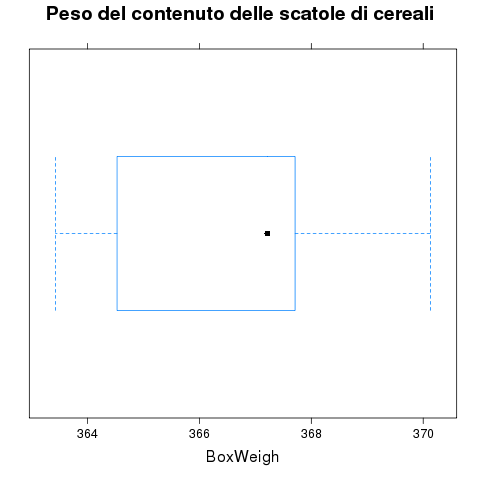
\includegraphics[width=6cm]{14_10.png}
  \end{center}
\end{frame}

\begin{frame}[fragile]
  Computation of Z test:
  \begin{verbatim}
Z = 1.7396, p-value = 0.08192
alternative hypothesis: true mean is not equal to 365
95 percent confidence interval:
 364.7841 368.6249
sample estimates:
mean of x: 366.7045
  \end{verbatim}
\end{frame}

\begin{frame}[fragile]
  Computation of t test:
  \begin{verbatim}
t = 1.7375, df = 5, p-value = 0.1428
alternative hypothesis: true mean is not equal to 365
95 percent confidence interval:
 364.1828 369.2262
sample estimates:
mean of x: 366.7045
  \end{verbatim}
\end{frame}

\begin{frame}
  \begin{itemize}
    \item According to tests Z there is no evidence that the current process does not respect the parameters expected.
    \item The t-test confirms this result.
    \item The two tests give a different value of p-value: in particular the p-value of Z  test is lower than that of the t test. This is due to the fact that the t test has a reference distribution ($t_{5}$) much more dispersed than the Z test ($N(0,1)$). As the value of Z test and of t test are nearly equal, the probability to obtain ``outer'' values to the value of the test will be higher for the  more dispersed distribution.
    \item As a consequence of this statement, also the confidence interval computed under the hypothesis of knowing the standard deviation value of data results to be more ``tight'' than that computed under the hypothesis of not knowing the standard deviation value. 
  \end{itemize}
\end{frame}

\livelloB{Check the milk quality}

\begin{frame} 
  \begin{description}
    \item[Data:] cheese.txt\\ 
      Data of the freezing temperature of the milk supply.
    \item[Aims:] \begin{small}A cheese factory receives milk from its suppliers. The owner suspects that milk received from one of the suppliers is ``watered down''. To check that, he collects milk samples and he checks the characteristics measuring the freezing temperature. If the milk is ``good'', It should freeze at a temperature on average not higher than -0.545$^o$C.\end{small}  
      \begin{itemize} \begin{small}
        \item[-] Let us compute the main descriptive statistics and let us graphically summarise data.
        \item[-] Let us try to check the if the average temperature is not higher than -0.545$^o$C against if It is.
        \item[-] Let us try to apply a two-sided test. What are the results? Why is there a difference?
        \item[-] Let us compute the 95\% confidence interval of the mean in both cases.
      \end{small}\end{itemize}
  \end{description}
\end{frame}

\begin{frame}
  Computation of descriptive statistics and B-W graphic:\\
  \vspace{.3cm}
  \begin{scriptsize}
    \begin{tabular}{|l|rrrrrrr|}
      \hline
      & \textbf{Min}. & 1\textbf{st.Qu}. & \textbf{Median} & \textbf{Mean} & \textbf{3rd.Qu.} & \textbf{Max.} & \textbf{Sd}\\
      \hline
      \textbf{FrzTemp(N=10)} & -0.5562 & -0.5427 & -0.5381 & -0.5394 & -0.5335 & -0.5311 & 0.0078\\
      \hline	
    \end{tabular}
  \end{scriptsize}
  \begin{center}
    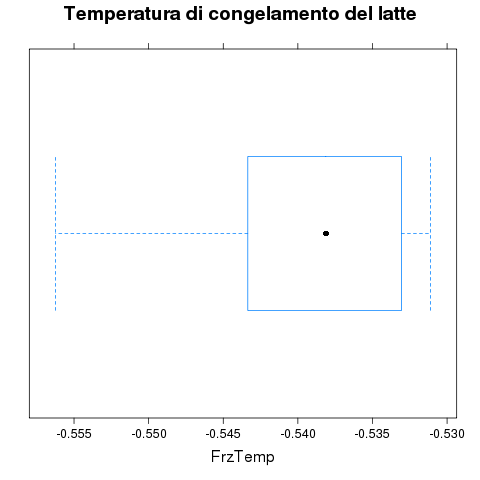
\includegraphics[width=6cm]{14_11.png}
  \end{center}
\end{frame}

\begin{frame}[fragile]
  Computation of t test (unilateral hypothesis):
  \begin{verbatim}
t = 2.2835, df = 9, p-value = 0.02414
alternative hypothesis: true mean is greater than -0.545
95 percent confidence interval:
 -0.5438892        Inf
sample estimates:
mean of x: -0.5393685
  \end{verbatim}
\end{frame}

\begin{frame}[fragile]
  Computation of t test (bilateral hypothesis):
  \begin{verbatim}
t = 2.2835, df = 9, p-value = 0.04828
alternative hypothesis: true mean is not equal to -0.545
95 percent confidence interval:
 -0.5449473 -0.5337897
sample estimates:
mean of x: -0.5393685
  \end{verbatim}
\end{frame}

\begin{frame}
  \begin{itemize}
    \item The unilateral test rejects the hypothesis that the milk is not watered down.
    \vspace{0.75cm}
    \item Also the bilateral test rejects this hypothesis, but with a p-value very close to 0.05; so It obtains a ``borderline'' result.
    \vspace{0.75cm}
    \item The difference between the two tests is found only on the value of the p-value; all the others statistics (apart from the confidence intervals) are equal.
  \end{itemize}
\end{frame}

\livelloB{Ball bearings diameter}

\begin{frame} 
  \begin{description}
    \item[Data:] bearings.txt\\ 
      Data on the measurements of the ball bearings diameter.
    \item[Aims:]
      \begin{small}
        A mechanical firm produces ball bearings. From past experience, It is known that the standard deviation of the diameter measurements is about 0.004 cm. 10 bearings have been collected to check the hypothesis that the mean value is equal to 0.5 cm. 
        \begin{itemize}
          \item[-] Let us compute the main descriptive statistics and let us graphically summarise  the data.
          \item[-] Let us check the hypothesis that the mean diameter is 0.5 cm against the hypothesis that It is not using Z and t test.
          \item[-] Let us compute the 95\% confidence interval for the mean in both cases.
          \item[-] Let us check the hypothesis of normality of the data using Normal Probability Plot and A-D test. 
        \end{itemize}
      \end{small}
  \end{description}
\end{frame}

\begin{frame}
  Computation of descriptive statistics and B-W graphic:\\
  \vspace{.3cm}
  \begin{scriptsize}
    \begin{tabular}{|l|rrrrrrr|}
      \hline
      & \textbf{Min}. & 1\textbf{st.Qu}. & \textbf{Median} & \textbf{Mean} & \textbf{3rd.Qu.} & \textbf{Max.} & \textbf{Sd}\\
      \hline
      \textbf{Bearings(N=10)} & 0.5003 & 0.5051 & 0.5069 & 0.5072 & 0.509 & 0.5154 & 0.0041\\
      \hline	
    \end{tabular}
  \end{scriptsize}
  \begin{center}
    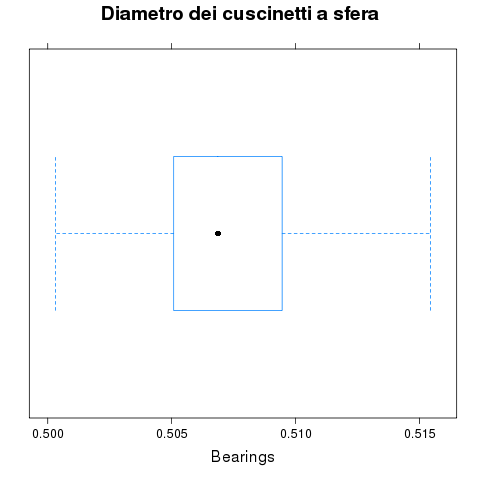
\includegraphics[width=6cm]{14_12.png}
  \end{center}
\end{frame}

\begin{frame}[fragile]
  Computation of Z test:
  \begin{verbatim}
Z = 5.6727, p-value = 0.0000
alternative hypothesis: true mean is not equal to 0.5
95 percent confidence interval:
 0.50470 0.50965 
sample estimates:
mean of x: 0.50717
  \end{verbatim}
\end{frame}

\begin{frame}[fragile]
  Computation of t test:
  \begin{verbatim}
t = 5.476, df = 9, p-value = 0.0003922
alternative hypothesis: true mean is not equal to 0.5
95 percent confidence interval:
 0.5042113 0.5101397
sample estimates
mean of x: 0.5071755
  \end{verbatim}
\end{frame}

\begin{frame}
  Computation of normality test:\\
  \texttt{A = 0.2234, p-value = 0.7602}
  \vspace{.3cm}
  \begin{center}
    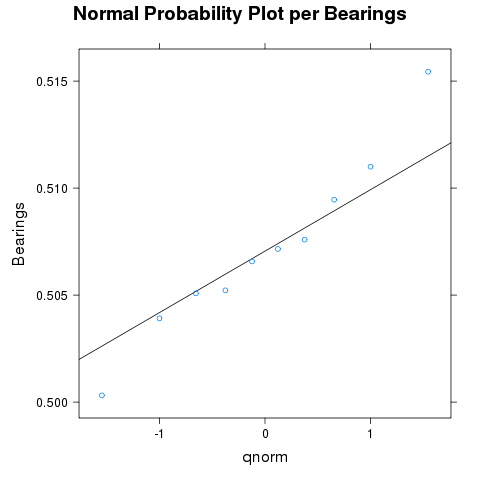
\includegraphics[width=6cm]{14_13.png}
  \end{center}
\end{frame}

\begin{frame}
  \begin{itemize}
    \item The diameter values of the ball bearings is rather stable, with standard deviation close to the expected values.
    \vspace{0.5cm}
    \item The average of the sampled diameter values doesn't seem to be compatible with the hypothesized value of 0.5cm: both Z test and t test reject the null hypothesis.
    \vspace{0.5cm}
    \item Both tests are reliable because the normal probability plots and the Anderson-Darling tests confirm the hypothesis of normality for observed data.
  \end{itemize}
\end{frame}

\livelloB{Comparison of two suppliers of plastics}

\begin{frame} 
  \begin{description}
    \item[Data:] plastic.txt\\ 
      Two columns of measurement data of resistance for wafer plastic of two suppliers.
    \item[Aims:] 
      \begin{small}
        Two companies provided plastic wafer to compare the performance of resistance (measured in Newton).
        \begin{itemize}
          \item[-] Let us compute the main descriptive statistics and let us graphically summarise data of both companies.
          \item[-] Let us check the hypothesys that the mean resistance of the two products is fundamentally the same.
          \item[-] Let us check the hypothesis that the variability of the resistance of the two products is fundamentally the same.
          \item[-] Let us check the hypothesis of normality of data using Normal Probability Plot and A-D test. 
          \item[-] What conclusions can be drawn to the medium? And for the variability?
        \end{itemize}
      \end{small}
  \end{description}
\end{frame}

\begin{frame}
  Computation of descriptive statistics and B-W graphic:\\
  \vspace{.3cm}
  \begin{scriptsize}
    \begin{tabular}{|l|rrrrrrr|}
      \hline
      & \textbf{Min}. & 1\textbf{st.Qu}. & \textbf{Median} & \textbf{Mean} & \textbf{3rd.Qu.} & \textbf{Max.} & \textbf{Sd}\\
      \hline
      \textbf{SupplrA(N=20)} & 151.8 & 160.8 & 165 & 163.8 & 167.2 & 175.6 & 5.66\\
      \textbf{SupplrB(N=20)} & 152.7 & 157.8 & 161 & 160.0 & 162.2 & 165.0 & 3.23\\
      \hline	
    \end{tabular}
  \end{scriptsize}
  \begin{center}
    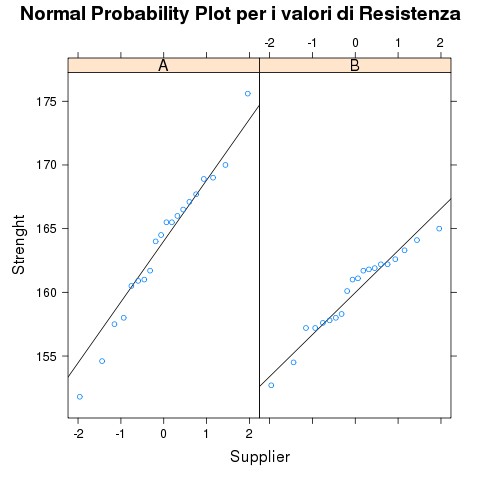
\includegraphics[width=6cm]{14_14.png}
  \end{center}
\end{frame}

\begin{frame}[fragile]
  Computation of t test:
  \begin{verbatim}
data:  SupplrA and SupplrB
t = 2.2651, df = 30.168, p-value = 0.03085
alternative hypothesis:
  true difference in means is not equal to 0.5
95 percent confidence interval:
 0.8252722 6.7747278
sample estimates:
mean of x: 163.815 mean of y: 160.015 
  \end{verbatim}
\end{frame}

\begin{frame}[fragile]
  Check of the equality of variances (F or Bartlett test):
  \begin{verbatim}
F = 3.0777, num df = 19, denom df = 19, p-value = 0.01831
alternative hypothesis: 
  true ratio of variances is not equal to 1 
95 percent confidence interval:
 1.218190 7.775652 
sample estimates: ratio of variances = 3.077698 
  \end{verbatim}
  \vspace{.2cm}
  Check of the equality of variances (Levene test):\\
  \begin{tabular}{l|rrrr}
    \hline
    & \texttt{Df} & \texttt{F value} & \texttt{p-value} \\
    \hline
    \texttt{group} & \texttt{1} & \texttt{3.5557} & \texttt{0.067} \\
    & \texttt{38} & & & \\
    \hline
  \end{tabular} 
\end{frame}

\begin{frame}
  Computation of normality test:\\
  \vspace{.3cm}
  \begin{scriptsize}
    \begin{tabular}{ll}
      \textbf{SupplrA} & \textbf{SupplrB}\\
      \texttt{A = 0.2474, p-value = 0.7179} & \texttt{A = 0.4927, p-value = 0.1928}\\
    \end{tabular} 
  \end{scriptsize}
  \begin{center}
  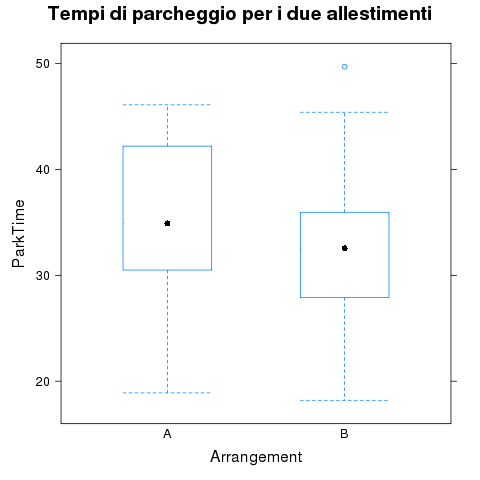
\includegraphics[width=6cm]{14_15.png}
  \end{center}
\end{frame}

\begin{frame}
  \begin{itemize}
    \item Two-sample t test, for the check of the hypothesis of equality of the averages, doesn't confirm this hypothesis.
    \vspace{0.3cm}
    \item Test to check the equality of the variances of the two suppliers provides conflicting results: Bartlett (or F) Test, which is based on the assumption of the normality of data, asserts that there are significant differences, however the Levene Tets (more robust) doesn't find evidence of rejecting the hypothesis of equality of variance.
    \vspace{0.3cm}
    \item As the normal probability plot and the Andreson-Darling test confirm the hypothesis of normality for observed data, It is possible to conclude that both t test and Bartlett test are valid. However, It is still better to accept carefully the results of the second.
  \end{itemize}
\end{frame}



\livelloA{Paired t test}

\livelloB{Parking time of two different car equipments}

\begin{frame} 
  \begin{description}
    \item[Data:] carctl.txt\\ 
      Comparison between the parking time of a same car with two different equipments.
    \item[Aims:]
      \begin{small}
        The aim is to check if the parking time of a same car with two different equipment are equal in average. Both cars were parked by 20 drivers, and the related times are collected (a row for each driver parking). The trials are randomized.  
        \begin{itemize}
          \item[-] Let us compute the main descriptive statistics and let us graphically summarise data of both equipments.
          \item[-] Let us check the hypothesis that the parking time of the two equipments is the same.
          \item[-] What test was used? Why?
          \item[-] Let us to check the hypothesis of normality of data using Normal Probability Plot and A-D test. 
        \end{itemize}
      \end{small}
  \end{description}
\end{frame}

\begin{frame}
  Computation of descriptive statistics and B-W graphic:\\
  \vspace{.3cm}
  \begin{scriptsize}
    \begin{center}
      \begin{tabular}{|l|rrrrrrr|}
        \hline
        & \textbf{Min}. & 1\textbf{st.Qu}. & \textbf{Median} & \textbf{Mean} & \textbf{3rd.Qu.} & \textbf{Max.} & \textbf{Sd}\\
        \hline
        \textbf{Car\_A(N=20)} & 18.9 & 30.75 & 34.90 & 34.86 & 42.20 & 46.1 & 7.59\\
        \textbf{Car\_B(N=20)} & 18.2 & 28.25 & 32.55 & 32.90 & 35.92 & 49.7 & 7.27\\
        \hline	
      \end{tabular}
      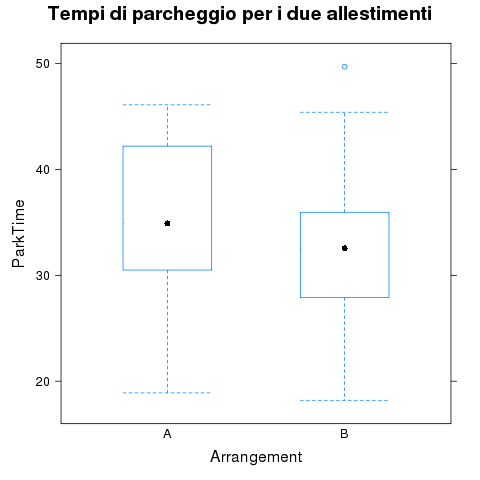
\includegraphics[width=6cm]{14_16.png}
    \end{center}
  \end{scriptsize}
\end{frame}

\begin{frame}[fragile]
  Computation of paired t test (t-test for differences):\\
  \begin{verbatim}
t = 2.2911, df = 19, p-value = 0.03356
alternative hypothesis: true mean is not equal to 0
95 percent confidence interval:
 0.1698814 3.7601186
sample estimates:
mean of x: 1.965  
  \end{verbatim}
\end{frame}

\begin{frame}
  Computation of normality test:\\
  \vspace{.3cm}
  \begin{scriptsize}
    \begin{tabular}{ll}
      \textbf{Car\_A } & \textbf{Car\_B}\\
      \texttt{A = 0.3239, p-value = 0.5038} & \texttt{A = 0.2855, p-value = 0.589}\\
    \end{tabular} 
  \end{scriptsize}
  \begin{center}
  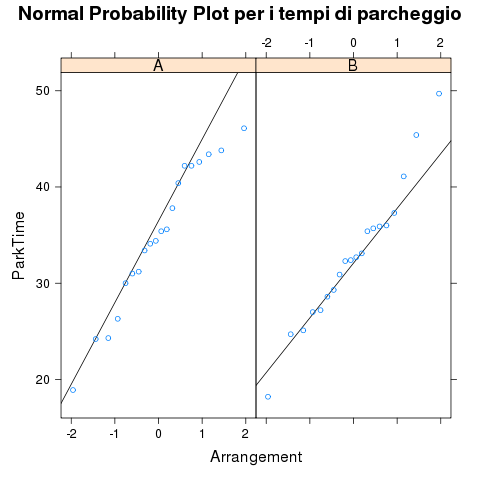
\includegraphics[width=6cm]{14_17.png}
  \end{center}
\end{frame}

\begin{frame}[fragile]
Computatio of two-sample t test:\\
  \begin{verbatim}
t = 0.8358, df = 37.931, p-value = 0.4085
alternative hypothesis: 
  true difference in means is not equal to 0
95 percent confidence interval:
 -2.794713  6.724713
sample estimates:
mean of x: 34.865   mean of y: 32.900
  \end{verbatim}
\end{frame}

\begin{frame}
  \begin{itemize}
    \item The paired t test highlight a significant difference between the two equipments.
    \vspace{0.4cm}
    \item The equipment A seems to produce longer parking times.
    \vspace{0.4cm}
    \item The check for normality of data confirms the possibility of using t test.
    \vspace{0.4cm}
    \item If an unpaired t test was used, It would obtain a non significant difference between averages.  
  \end{itemize}
\end{frame}

\livelloB{pH measure tools}

\begin{frame} 
  \begin{description}
    \item[Data:] labtest.txt\\ 
      Comparison between the pH measure tools on the same samples of material.
    \item[Aims:]
      \begin{small}
        The aim is to check if the two instruments (in lab and ``on the field'') don't give systematic differences measuring the same samples. 
        \begin{itemize}
          \item[-] Let us check the hypothesis that the two tools don't give systematic differences measuring the same samples.
          \item[-] What test was used? Why?
          \item[-] Let us to check the hypothesis of normality of data using Normal Probability Plot and A-D test. 
          \item[-] Are two ``interchangeable'' tools, considering also the previous evaluation on the same data?
        \end{itemize}
      \end{small}
  \end{description}
\end{frame}

\begin{frame}
  Computation of descriptive statistics and B-W graphic:\\
  \vspace{.3cm}
  \begin{scriptsize}
    \begin{center}
      \begin{tabular}{|l|rrrrrrr|}
        \hline
        & \textbf{Min}. & 1\textbf{st.Qu}. & \textbf{Median} & \textbf{Mean} & \textbf{3rd.Qu.} & \textbf{Max.} & \textbf{Sd}\\
        \hline
        \textbf{Lab(N=20)} & 8.6 & 8.95 & 9.05 & 9.025 & 9.100 & 9.4 & 0.1916\\
        \textbf{Online(N=20)} & 8.7 & 9.00 & 9.20 & 9.170 & 9.225 & 9.6 & 0.2105\\
        \hline
      \end{tabular}
      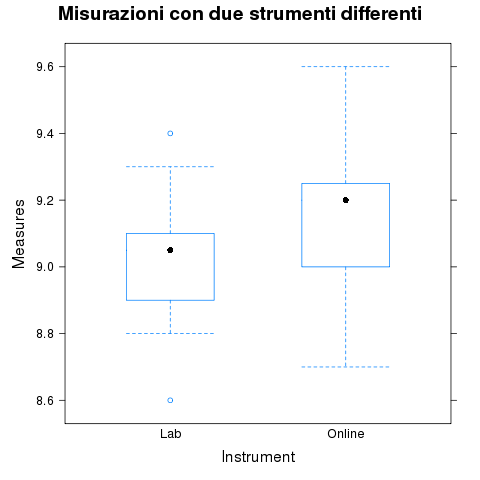
\includegraphics[width=6cm]{14_18.png}
    \end{center}
  \end{scriptsize}
\end{frame}

\begin{frame}[fragile]
  Computation of paired t test (t-test for differences):\\
  \begin{verbatim}
t = -10.7218, df = 19, p-value = 1.693e-09
alternative hypothesis: true mean is not equal to 0
95 percent confidence interval:
 -0.1733058 -0.1166942
sample estimates:
mean of x: -0.145
  \end{verbatim}
\end{frame}

\begin{frame}
  Computation of the normality test:\\
  \vspace{.3cm}
  \begin{scriptsize}
    \begin{tabular}{ll}
      \textbf{Lab } & \textbf{Online}\\
      \texttt{A = 0.6207, p-value = 0.09116} & \texttt{A = 0.4793, p-value = 0.2087}\\
    \end{tabular} 
  \end{scriptsize}
  \begin{center}
    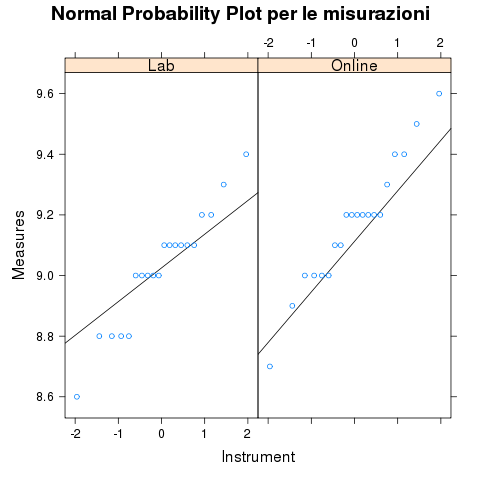
\includegraphics[width=6cm]{14_19.png}
  \end{center}
\end{frame}

\begin{frame}[fragile]
  Computation of two-sample t test:\\
  \begin{verbatim}
t = -2.2781, df = 37.668, p-value = 0.02848
alternative hypothesis: 
  true difference in means is not equal to 0
95 percent confidence interval
 -0.27388987 -0.01611013
sample estimates:
mean of x: 9.025 mean of y: 9.170 
  \end{verbatim}
\end{frame}

\begin{frame}[fragile]
  Check of the equality of variances (F or Bartlett test):
  \begin{verbatim}
F = 0.8284, num df = 19, denom df = 19, p-value = 0.6857
alternative hypothesis:
  true ratio of variances is not equal to 1
95 percent confidence interval:
 0.3278848 2.0928735
sample estimates:
ratio of variances: 0.8283848
  \end{verbatim}
   Check of the equality of variances (Levene test):\\
  \begin{tabular}{l|rrrr}
    \hline
    & \texttt{Df} & \texttt{F value} & \texttt{p-value} \\
    \hline
     \texttt{group} & \texttt{1} & \texttt{0.0136} & \texttt{0.9078} \\
     & \texttt{38} & & & \\
    \hline
  \end{tabular} 
\end{frame}

\begin{frame}
  \begin{itemize}
    \item The paired t test highlight a significant difference between the two equipments.
    \item The laboratory tool (Lab) seems to produce measurements systematically lower than the Online tool.
    \item The check for normality of data confirms the possibility of using the t test, even if the NPP doesn't seem to be ``beautiful''.
    \item Also unpaired t test highlight differences, even if the application of this method is not methodologically correct.
    \item The test for the check of equality of variances, even if It is not required, doesn't seem to highlight evident differences between the two tools.
  \end{itemize}
\end{frame}

\livelloA{P and Chi-Squared Test}

\livelloB{Analysis on one proportion}

\begin{frame} 
  Check on the pencentage of defectiveness water filters for air conditioners.
  \begin{description}
    \item[Aims:]
      \begin{small}
        The aim is to check if the number of defective pieces produced by a company that produces water filters for air conditioners is less than or equal to 2\%, against the hypothesis that It is greater than 2\%. 
        \begin{itemize}
          \item[-] Let us to check the hypothesis that the percentage of defective pieces could be less or equal to 2\%, knowing that from a sample of 500 filters collected, 18 are defective.
          \item[-] What will be the `` real minimum '' percentage compatible with the extracted data?
        \end{itemize}
      \end{small}
  \end{description}
\end{frame}

\begin{frame}[fragile]
  Computation of test for one proportion with unilateral alternative hypothesis: 
  \begin{verbatim}
number of successes = 18
number of trials = 500
p-value = 0.01339
alternative hypothesis: 
  true probability of success is greater than 0.02
95 percent confidence interval:
 0.02339513 1.00000000
sample estimates:
probability of success: 0.036 
  \end{verbatim}
\end{frame}

\begin{frame}
  \begin{itemize}
    \item The test for one proportion highlighted a discordance between the expected value and the observed number of defective pieces: the null hypothesis is not accepted.
    \vspace{0.75cm}
    \item The test has been performed using an unilateral alternative hypothesis.
    \vspace{0.75cm}
    \item The 95\% lower bound for the real proportion of defective pieces is about 2.34\%.
  \end{itemize}
\end{frame}

\livelloB{Analysis of two proportions}

\begin{frame} 
   Check on the pencentage of defectiveness water filters for air conditioners.
  \begin{description}
    \item[Aims:]
      \begin{small}
        The previous test highlights a significant difference between the percentage of expected defectiveness and that observed. The aim is to check if changing glue the percentage decreases significantly. So, other 100 filters with the new glue was studied, without finding any defective piece.  
        \begin{itemize}
          \item[-] Let us check the hypothesis that the percentage of defective pieces with the new glue is significantly different than that observed with the old glue.
        \end{itemize}
      \end{small}
  \end{description}
\end{frame}

\begin{frame}[fragile]
Computation of the test for two proportion with bilateral alternative:\\
  \begin{verbatim}
X-squared = 2.5773, df = 1, p-value = 0.1084
alternative hypothesis: two.sided
95 percent confidence interval:
 0.01367125 0.05832875
sample estimates:
prop 1 prop 2
 0.036  0.000
  \end{verbatim}
\end{frame}

\begin{frame}
  \begin{itemize}
    \item The test for two proportion confirms the hypothesis that two subsamples could belong to the same population: It is accepted the null hypothesis of equality of proportion. 
    \vspace{0.75cm}
    \item The test was performed using the bilateral alternative hypothesis.
    \vspace{0.75cm}
    \item The real value of the proportion will be included between l'1.367\% e il 5.833\%, with 95\% confidence level.
  \end{itemize}
\end{frame}

\livelloB{Comparison between adjusted and non adjusted productive process}

\begin{frame} 
  \begin{description}
    \item[Data:] adjust.txt\\
    Let us use the same data already seen previously to analyse if the differences between the percentage of pieces out specification are significantly different for the adjusted process and for the non adjusted process.
  \end{description}
  \begin{center}
    \begin{tabular}{|l|rr|c|l|rr|}
      \hline	
      \textbf{AdjustIn} & \textbf{No} & \textbf{Yes} & & \textbf{NoAdjustIn} &  \textbf{No} & \textbf{Yes} \\
      \hline
      \textbf{Counts} & 12 & 38 & & \textbf{Counts} & 3 & 47 \\
      \textbf{\%} & 24\% & 76\% & & \textbf{\%} & 6\% & 94\% \\
      \hline
    \end{tabular} 
    \end{center}
\end{frame}

\begin{frame}[fragile]
Let us check the hypothesis that the two processes (adjusted and not) have the same proportion of pieces out of specification, against the alternative hypothesis that the adjusted process has a lower percentage of pieces out of specification than the non adjusted process.
  \begin{verbatim}
data:  c(38, 47) out of c(50, 50) 
X-squared = 5.0196, df = 1, p-value = 0.01253
alternative hypothesis: less 
95 percent confidence interval:
 -1.00000000 -0.04632645 
sample estimates:
prop 1 prop 2 
  0.76   0.94 
  \end{verbatim}
\end{frame}

\begin{frame}[fragile]
Let us check the hypothesis that the two processes (adjusted and not) have the same proportion of pieces out of specification, against the alternative hypothesis that they have a different percentage.
  \begin{verbatim}
data:  c(38, 47) out of c(50, 50) 
X-squared = 5.0196, df = 1, p-value = 0.02506
alternative hypothesis: two.sided 
95 percent confidence interval:
 -0.33545039 -0.02454961 
sample estimates:
prop 1 prop 2 
  0.76   0.94
  \end{verbatim}
\end{frame}

\livelloB{Analysis of the data of the Titanic passengers}

\begin{frame} 
  \begin{description}
    \item[Data:] titanic.txt\\ 
      Percentage of survived passengers for sex, class of travel and age
    \item[Aims:]
      \begin{small}
        Data concern personal and travel informations of the single passengers, as well as their survival. The aim is to determine if there are differences in survival probability by varying the class of travel and by varying the sex of the passenger.  
        \begin{itemize}
          \item[-] Let us compute the survival percenatge for sex and class of travel.
          \item[-] Let us check if the survival probability is equal for the two classes of travel.
          \item[-] Let us check if the survival probability is equal for the two sexes.
        \end{itemize}
      \end{small}
  \end{description}
\end{frame}

\begin{frame}
  Frequency tables and survival percentage for classes of travel:\\
  \begin{center}
    \begin{tabular}{|l|rr|c|l|rr|}
      \hline	
      & \textbf{Died} & \textbf{Survived} & &  &  \textbf{Died} & \textbf{Survived} \\
      \hline
      \textbf{Coach} & 1368 & 508 & & \textbf{Coach} & 72.9\% & 27.1\% \\
      \textbf{First} & 122 & 203 & & \textbf{First} & 37.5\% & 62.5\% \\
      \hline
    \end{tabular} 
  \end{center}
  Frequency tables and survival percentage for sex:
  \begin{center}
    \begin{tabular}{|l|rr|c|l|rr|}
      \hline	
      & \textbf{Died} & \textbf{Survived} & &  &  \textbf{Died} & \textbf{Survived} \\
      \hline
      \textbf{Female} & 126 & 344 & & \textbf{Female} & 26.8\% & 73.2\% \\
      \textbf{Male} & 1364 & 367 & & \textbf{Male} & 78.8\% & 21.2\% \\
      \hline
    \end{tabular} 
  \end{center}
\end{frame}

\begin{frame}[fragile]
  Computation of the test for two proportions to check the survival probabilities for the two classes of travel:\\
  \begin{verbatim}
X-squared = 413.0191, df = 2, p-value < 2.2e-16
alternative hypothesis: two.sided
null values:
prop 1 prop 2
   0.5    0.5
sample estimates:
   prop 1    prop 2
0.7292111 0.3753846 
  \end{verbatim}
\end{frame}

\begin{frame}[fragile]
Computation of the test for two proportions to check the survival probabilities for the two sexes:\\
  \begin{verbatim}
X-squared = 673.2777, df = 2, p-value < 2.2e-16
alternative hypothesis: two.sided
null values:
prop 1 prop 2 
   0.5    0.5
sample estimates:
   prop 1     prop 2
0.2680851  0.7879838
  \end{verbatim}
\end{frame}

\begin{frame}
  \begin{itemize}
    \item The percentage of survived passengers for class of travel and for sex are very different from the expected values, that is .5. 
    \vspace{0.75cm}
    \item Both the test for the check of equality of survival percentage between classes of travel, and that for the check of equality between the percentage of sex categorically reject this hypothesis.
    \vspace{0.75cm}
    \item The survival probability is much higher for women and for first class passengers.
  \end{itemize}
\end{frame}


